\documentclass[main.tex]{subfiles}

\begin{document}

 \notinmain{ka ble ikke gjort/kva må bli gjort i fremdtiden, hvordan kan system bli gjenbrukt til readout electronics og cooling}

\section{Discussion}
\textit{This chapter describes the functionality of the control software created in this thesis, what is complete and what is missing. The chapter covers missing features and how the software can be expanded in the future. A discussion is made on the system's modularity and how we can repurpose it within the PCT project.}

\subsection{Reusability}
 
 The configuration and monitoring systems developed in this thesis have been built using software design standards to make it generic and modular. The system is layered in such a manner that individual parts with specific functions can be reused in other systems. This section discusses how these parts can be reused.
 
 \subsubsection{Monitoring software}
The monitoring software is comprised of \textit{influx\_api}, \textit{configuration\_api}, and \textit{panda\_filter}. The influx API class requires very little modification to be used in other systems. The \gls{api} has functions for inserting values into the database, and for filtering data points with the \textit{panda\_filter} class. Certain tags in the class must be redefined to match the new system it interfaces with, i.e. change "layer" to "flowmeter", for example.

The panda filter class uses pandaframe to filter received data. It currently is only capable of filtering data based on the exception process described in \autoref{ssec: downsampling}, but additional functions can be created to perform other filters on the data.

The monitoring \gls{api} does not require any direct modification to be repurposed to another system, but it requires a lower level \gls{api} to interface with, akin to the microcontroller \gls{api}. The \textit{monitor\_addr} list must also be edited to include the desired registers to poll.

\subsubsection{Configuration software}

The configuration software is comprised of \textit{db\_manager}, and \textit{configuration\_api}. The configuration \gls{api} is specialized to configure, and power on the \gls{pcs}; the configuration functions must therefore be reworked for other systems. \autoref{ssec: power_algo} shows that the configuration process is in two stages, stage 1 configures general registers, and stage 2 performs the ramp-up algorithm. Stage 1 may be suitable to reuse since it only performs basic write operations. However, stage 1 also contains system-specific functions, such as handshake verification, that must be removed or modified.

The \textit{db\_manager} is the interface between the Python classes and MongoDB. It is relatively simple; its primary function is to create configuration sets for the \gls{pcs}. The configuration sets store single values for most registers, but the threshold 2 registers have individual values for each string. This formatting must be revised or removed if we reuse the manager to create configuration sets in the future. 

The lower level \gls{api}s that connect to the microcontroller and the MB Hub uses IPbus to communicate, and other systems that use IPbus can base their design on these \gls{api}s. The readout system, in particular, uses IPbus for configuring the ALPIDE-sensors, and therefore could base its structure on the Power Control System \gls{api}. The cooling system reads out data using Moxa modules, not IPbus, which means the lower level \gls{api} must be redefined, but it could still utilize the same concepts, such as having multiple levels of \gls{api} abstraction.
 
 \subsubsection{Register Package}
 
The \gls{api}s developed for the \gls{pcs} use namedtuples to process register information, which is described in \autoref{ssec: mcu_api}. The namedtuples make it easier to repurpose the \gls{api}s to a different system. A developer can define the address map of a different module using the same namedtuples, and the \gls{api}s would only require small modifications to work with the new system.



\subsection{Error handling}

\subsubsection{Control Software}

The error handling from the control software is not finalized. By "errors," we refer to the microcontroller's error messages, which are discussed in \autoref{ssec: microcontroller}. Currently, only the monitoring system checks for errors during its polling function. The error handling design has not been decided yet, but this section will go over potential implementations.

The configuration and monitoring systems require functions to retrieve error messages. This suggests that an "Error Manager" class should be developed, which contains general functions for handling the errors. Both the configuration and monitoring \gls{api}s could use this manager to handle errors, reducing redundant code in the \gls{api}s and increasing the software's modularity.

A design choice must be made on storing and displaying the microcontroller's errors. Ideally, the error messages should be stored in a logging database and displayed to the user, but that design decision has not been made yet. Currently, the error messages are not stored, only displayed in the monitoring \gls{gui}. InfluxDB could store the logging information, and separate tags could indicate each error's severity. Another option for handling logging is Grafana Loki, a log aggregation system that is optimized for Grafana. 

\subsubsection{Microcontroller}
The microcontroller software supports custom control functions that can be performed by writing to the control registers on the microcontroller. Utilizing these custom functions could reduce the number of transmissions needed for error handling, increasing the speed of the error handling algorithm. For example, identifying faulty strings would be a cumbersome process for the control software; turning on the strings to test their current consumption individually would require multiple transmissions through the entire \gls{pcs}-chain. A microcontroller function that automatically turns each stave on, one by one, and then measures their current consumption would make the process significantly faster. The control software would only need to call the function by writing to a register, retrieve the current values for each string, and compare them to the expected ones.

\subsection{Configuration System}

Currently, the broadcast function in the MB Hub is not used in the configuration process. This is due to the structure of the database; the database stores values for every layer. Using the broadcast functionality would require a separate function that checks if a register value is the same for every layer. If yes, broadcast the data; if not, it must configure the layers separately. This process would not only be cumbersome work, but it could potentially add more delay in the form of software overhead.

It is therefore required to restructure the database to use the broadcast function effectively. A possible solution is using a "default" configuration set in the database. For example, we would have a single configuration set that is used to configure all layers; however, each layer has an exception list, which overrides the default set. The default set is merged with the exception values, creating the final configuration set. A figure of the possible implementation of a default configuration set is given in \autoref{fig: default_database}.

\begin{figure}[!ht]
    \centering
    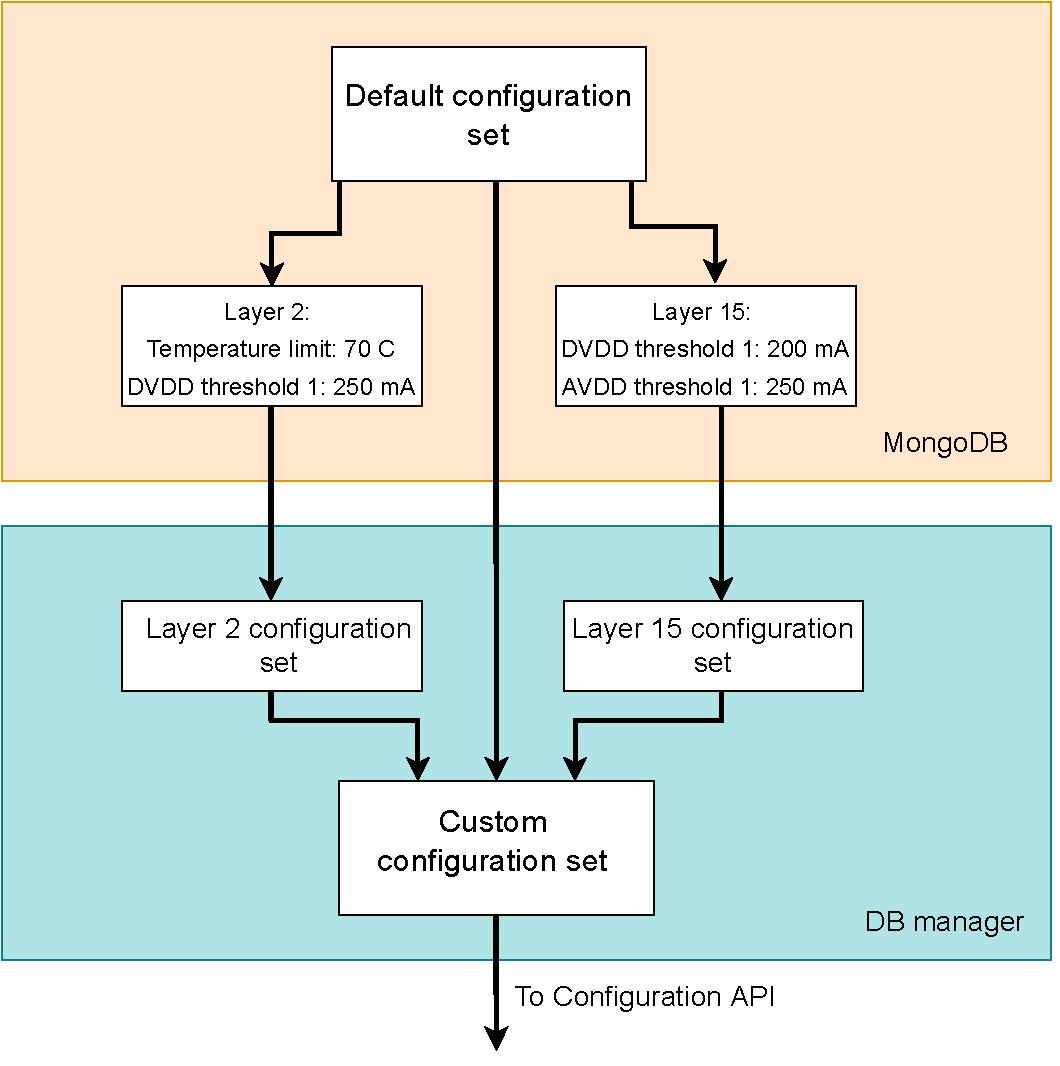
\includegraphics[scale=0.55]{images/default_database.pdf}
    \caption{Block diagram showing the implementation of a "default" configuration set in MongoDB.}
    \label{fig: default_database}
\end{figure}
\FloatBarrier 

The figure shows the default configuration set in the MongoDB database, exception lists for two layers, and the DB manager class retrieves the configuration set. DB manager will create a configuration set for each layer with an exception list and merge this configuration set with the default one, which gives us a custom configuration set. This custom set is sent to the configuration \gls{api}. Restructuring the database like this would also require changing the configuration \gls{api} to utilize the broadcast function.

The calculations and results from \autoref{ssec: con_timing} show that the configuration timing is already adequate for this project, only spending half a second to configure all layers. The default database presented in this section could be implemented in the future if timing becomes a problem.


 
 
\subsection{USART communication}

The communication link between the MB Hub and the microcontroller is outside the scope of this thesis. However, significant time has been spent on creating verification tests of the \gls{pcs}, and thus, by extension, includes the USART communication between the MB Hub and the microcontroller. This section covers the potential sources of the bit errors in the communication.

A 17 hour test was done on the USART communication in an earlier part of the development cycle, and no errors were observed. There were however errors observed at lower baud rates. The test setup was then briefly moved to an expo, and after returning, the error rate was observed to be much higher, similar to the results shown in \autoref{ssec: bit_error}, even at higher baud rates. These results suggest there exist two sources of errors in the communication, the first is dependent on the baud rate of the \gls{usart}, and the other is most likely caused by the inconsistent test environment. \notinmain{Skriv her mer om hva potensiellt er årasken til feilene etter at eg har omskrevet test kapittelet. Altså delta tid i baud rates og uneven ground levels.}

The source of the baud rate error is discussed in \autoref{ssec:baud_error}, where the conclusion was a $^\delta$t skew in the transmission for every clock cycle caused the errors, which was exacerbated with lower baud rates.

The results from \autoref{ssec: bit_error} showed that the bits always flipped from 0 to 1, never the other way around. This could hint what the error source might be, but no further tests have been done to uncover the error source. Previous tests of the prototype did not suffer from any errors in the bits, and as such, the most probable cause of the errors is the inconsistent test environment.

\subsection{Future work}

This section covers the remaining work on the system that should be done before it can be incorporated into the \gls{pct}-project.


\subsubsection{Docker Image}
 
 The control system uses several different packages and programs to function. The README file in the GitHub repository gives instructions on how to install all dependencies and run the program, but it is still cumbersome to move the system to a different computer. Therefore, a Docker Image of the system should be created in future work. Docker is a program that allows for building an "Image", a virtual environment for your program, containing all dependencies necessary to run the program. By building a Docker Image of a program, moving it to other computers only requires downloading a single docker file and running it.
 
 The main hub \gls{gui}, along with its lower level \gls{gui}s and \gls{api}s can all be encapsulated in one Docker Image. The databases and Grafana will most likely be located on different servers, therefore each of them should have their own Docker Image with their ports open to the \gls{gui} Image.

\subsubsection{Grafana}

The Grafana dashboard has four tabs for each measurement type: DVDD, AVDD, PWELL, and temperature. Each tab contains histograms for each layer, but it is currently impossible to display all tabs on one screen; this design may be cumbersome for the user. They must scroll through the tabs if they want to view multiple measurements simultaneously.

If the Grafana design is not satisfactory to the user in the future, a new dashboard design is warranted. A group of users should create this new design to ensure the dashboard is user-friendly.

\subsubsection{System parameters}

Currently, several system parameters is only defined as variables inside their respective classes. These parameters include ExDev, and ExMax, which affects the "exception" filtering process, and the batch size of the Influx API. It may be inconvenient for the user to edit many different files in order to change these parameters. The solution to this would be to have a separate "config" file, which contains parameter values that can be easily configured by the user. The "config" file could be implemtented in a simple text file, or possibly intergrated with the configuration database. The relevant classes would have to be changed to use the values from the "config" file.


 

\end{document}